\documentclass[12pt]{article}
% Set document indentation and font size

\author{Group 1}

% Packages for code block support
\usepackage{listings}
\usepackage{xcolor}
\usepackage{graphicx}
\usepackage{wrapfig}
\usepackage[utf8]{inputenc}
\usepackage[english]{babel}
\usepackage{amsfonts}
\usepackage{mathtools}          %loads amsmath as well
\DeclarePairedDelimiter\Floor\lfloor\rfloor
\DeclarePairedDelimiter\Ceil\lceil\rceil
\usepackage{amsmath}
\newcommand{\stirlingii}{\genfrac{\{}{\}}{0pt}{}}
\usepackage[a4paper, left=30mm, right=30mm, top=20mm, bottom=20mm]{geometry}
\usepackage{tikz}
\usepackage{pgfplots}
\pgfplotsset{compat=1.16}
\usepackage{setspace}
\setstretch{1.5}
\usepackage{indentfirst}
\usepackage{hyperref}
\usepackage[backend=biber, style=chicago-notes]{biblatex} 
\usepackage{booktabs}
\usepackage[utf8]{inputenc}
\addbibresource{bible.bib} 
\addbibresource{bible.bib}


% Define code block style
\lstset{
    language=Python, % Adjust based on the language you're including
    basicstyle=\small\sffamily,
    keywordstyle=\color{blue},
    commentstyle=\color{darkgray},
    stringstyle=\color{purple},
    backgroundcolor=\color{lightgray}, % Light gray background
    showspaces=false,
    showstringspaces=false,
    showtabs=false,
    frame=single,
    rulecolor=\color{black},
    tabsize=2,
    captionpos=b,
    breaklines=true,
    breakatwhitespace=true, % Only break lines at whitespaces
    framesep=3mm, % Space between frame and code
    lineskip=2pt, % Adjust line spacing for readability
    escapeinside={\%*}{*)},
}

%\setlength{\parindent}{0pt}

\newtheorem{theorem}{Theorem}[subsection] % Numbered as {sectionindex}.{subsection index}.{theorem number}
\newtheorem{lemma}{Lemma}[subsection] % Numbered within subsection
\newtheorem{definition}{Definition}[subsection] % Define the counter 'Definition'
\newtheorem{example}{Example}[subsection] % Define the counter 'Example'
\newtheorem{algorithm}{Algorithm}[subsection] % Define the counter 'Algorithm'
\newtheorem{corollary}{corollary}[subsection]
\newtheorem{proposition}{Proposition}
\newtheorem{remark}{Remark}


\begin{document}

\title{Group 1 Project Report}
\date{}

\maketitle
\newpage

\tableofcontents

\newpage

\section{Project Overview}
This project aims to generate a category list for a given wikipedia document. Instead of classical categorical model, we utilize probability mass function to construct for each category some probability mass function. The model is trained using wikipedia dataset, and the model is evaluated using cost function that is based on the difference between the actual category and the predicted category.\\

\newpage
\section{Model Description}
\subsection{Dataset}
Dataset is obtained from \href{https://www.kaggle.com/datasets/jjinho/wikipedia-20230701/data}{Kaggle}. The dataset is Wikipedia Plaintext obtained in 2023-07-01 Wikipedia dump. The dataset contains 6,826,775 articles, titles, text and categories from wikipedia. Dataset is provided in .parquet file, split per starting alphabet/character of the article title.

\subsection{Model Structure}
The model consist of largely 2 parts: Document Embedding and Category prediction. 
\subsubsection{Document Embedding}
Whilst many embedding method could be used, we utilized Bag of Words(Bow) method in our initial document embedding. BoW Encoder is first trained by obtaining unique words from all documents.\\
Unique words are obtained by first tokenizing the document. This is done using regex to replace all non-alphabet characters with whitespace, then split the document by whitespace. Afterwards, for each tokens stemming is applied for normalization.\\
However the unique words may not be entirely relevent. Unlike NLG tasks where no text can be dropped, we can eliminate tokens that have few relevence to our model.
\begin{itemize}
    \item \textbf{Stop Words} We use stop words provided from nltk package. Stop words are words in a stop list which are filtered out before or after processing of text. There is no universally agreed upon list of stop words due to nature of words that are irrelevant in one context may be relevant in another.
    \item \textbf{Least Frequency} We can also eliminate words that appear less than a certain threshold. This is done by counting the frequency of each word in the document and eliminating words that appear less than a certain threshold. In our project, we set the threshhold to 20.
    \item \textbf{tdf-idf Scoring} While nltk stopwords and least frequency are simple methods to eliminate irrelevant words, they are not perfect. tdf-idf scoring is a more advanced method to eliminate irrelevant words. tdf-idf scoring is a numerical statistic that is intended to reflect how important a word is to a document in a collection or corpus. The tdf-idf value increases proportionally to the number of times a word appears in the document and is offset by the number of documents in the corpus that contain the word. tdf-idf scoring is calculated by multiplying the term frequency and inverse document frequency. It can be represented as:\\
    For t:str=Token, d:list[str]=Document, D:list[d]=Documents\\
    \[
        tf(t,d) = \frac{f_{t,d}}{\sum_{d' \in D} f_{t,d'}}
    \]
    \[
        idf(t,D) = \log \frac{|D|}{|\{d \in D: t \in d\}|}
    \]
    \[
        tfidf(t,d,D) = tf(t,d) \times idf(t,D)
    \]
    This is simple method of tdf-idf scoring. However, in our project we used a variant of tf function called augmented frequency, which can be represented as:
    \[
        tf(t,d) = 0.5+0.5*\frac{f_{t,d}}{\max_{t' \in d} f_{t',d}}
    \]
    This is done to prevent bias towards longer documents.
\end{itemize}

Eliminating those tokens take place after all documents have been embedded using BoW embedder, as sort of post-processing.\\

\textbf{Dimension Reduction}
We used CUR decomposition for our project, processing 1500 rows per each bach to achieve the output dimension reduction of 1500.\\
CUR decomposition is a matrix decomposition method that is used to reduce the dimension of a matrix. It is similar to SVD decomposition,where CUR decomposition decomposes the matrix into three matrices. CUR decomposition is first selects subset of row and columns to be chosen to matrix C and R. Then, the matrix U is calculated as:
\[
    U = C^{-1}A R^{-1}
\]
Where A is approximated to minimize the difference.
CUR decomposition is used to reduce the dimension of sparse matrix where multiple elements are zero or close to zero.\\

\subsubsection{Category Prediction}
\textbf{Pmf Construction}\\
After document embedding,we construct a pmf for each category. After splitting the dataset into training and testing set, we calculate the probability of each word given the category.

Let $C$ the set of categories, $C_d, C_d'$ each the document category, and the forecasted category respectively. Then we can construct a base cost function as 
\[
    J(C_d, C_d') = \lambda_1|C_d'\setminus C_d| + \lambda_2|C_d\setminus C_d'|
\]
where $C_d$ is the set of categories in the document, $C_{d'}$ is the predicted set of categories. However this function will return different value range that is dependent on order of the sets $C_d, C_d'$, hence we can normalize it in form:
\[
    J_{norm}(C_d, C_d') = \frac{J(C_d, C_d')}{|C_d\cup C_d'|}
\]

While with other method $\lambda_1, \lambda_2$ may be also optimized, we can assume that $\lambda_1=\lambda_2=1$ for simplicity.\\

The process is as follows:
\begin{itemize}
    \item \textbf{Dataset Splitting}: We split the dataset into training and testing set. We use 70\% for training and 30\% for testing.
    \item \textbf{Category Clustering}: For each category, we filter all documents that have the category. Using distance metric, we can construct pmf using method above for each category.
    \item \textbf{Threshhold Optimization} After all pmf have been constructed, we adjust the pmf threashhold to optimize the cost function. This is done by adjusting the threshhold and calculating the cost function. The threshhold that results in the lowest cost function is selected.
\end{itemize}

\textbf{Prediction and Evaluation}

After model training, we predict the category of each document in the testing set. Then, using the cost function defined above, we can evaluate the model accuracy.

\newpage
\section{Model Implementation}
\subsection{Preprocessing}
Prior to implementing the model, the dataset was first filtered to only include categories that were related to history, science, art and literature. This was done because of large number of categories in the dataset, and the limited time and resource to train the model.\\
The category filtering was done by embedding all unique categories provided in the dataset, and embedding the words "history", "science", "art" and "literature" using openai text embedding model text-embedding-3-small. The cosine similarity between the embedded categories and the embedded words were calculated, and the categories with the highest similarity were selected.\\
The threshhold was set to 0.213 which resulted in filtering 98.9\% of the categories which resulted in reducing from 1,864,430 to 190,910 categories.\\
Afterward, dataset was filtered to only include documents that have at least one of the selected categories which resulted in approximately 33\% of data remaining.
\subsection{Document Embedding}
The documents were first embedded with BoW method described earlier, and least frequency was applied immediately within BoW training method with threshhold 20. This resulted in output dimension reduction from 1,859,340 to 323,658\\


\begin{wrapfigure}{r}{0.3\textwidth}
    \centering
    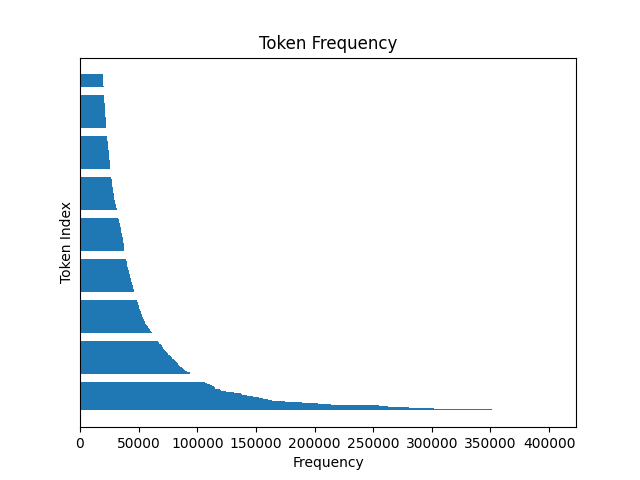
\includegraphics[width=0.5\textwidth]{bow_token_frequency.png}
    \caption{token frequency}
\end{wrapfigure}

After BoW model training, all document embedding vectors were summed to first analyze frequency of each words.

As seen in the figure, the frequency of each word looks similar to graph $y=\frac{1}{x}$, which is expected in natrual language according to Zipf's law.\\
Upon closer inspection, we can see that the most frequent tokens are tokens such as also, new, first, film... ect. While we can assume that those tokens might not be entirely relevent, it may differ per document context hence we apply tf-idf scoring to eliminate irrelevant tokens.\\

Originally tf-idf gives information score that is dependent on the given document. However, in this case what we're interested in is to eliminate irrelevent token, therefore for efficiency we've batched the data to 1500 rows where each row is a document, and we calculated the tf-idf score for each batch, for each tokens. Afterward, we summed the tf-idf score for each batch, and pruned the tokens using tf-idf score. Threshhold for tf-idf score was set to 30 through manual review, and after dropping tokens with less then 30 score, we were left with 95817 tokens, dropping 227841 tokens.\\

\subsection{Dimension Reduction}
From this point, we batched data to 1500 rows per batch, and applied CUR decomposition to reduce the dimension to 1500.\\
This was done using pytorch library for efficiency.

\end{document}